
\subsection{\label{sec:Tutorial-3d-hex8-gravity}Gravitational Body Force Examples}

PyLith features discussed in this tutorial:
\begin{itemize}
\item Gravitational body forces
\item Initial stresses
\item Finite strain
\item Generalized Maxwell linear viscoelastic material
\end{itemize}

\subsubsection{Overview}

This set of examples describes a set of problems for PyLith involving
gravitational body forces. All of the examples are quasi-static and
run for a time period of 200 years. These examples also demonstrate
the use of a generalized Maxwell viscoelastic material, which is used
for the lower crust in all examples. The final example (step17) demonstrates
the usage of a finite strain formulation, which automatically invokes
the nonlinear solver. All of the examples are contained in the directory
\texttt{examples/3d/hex8}, and the corresponding \texttt{.cfg} files
are \texttt{step15.cfg}, \texttt{step16.cfg}, and \texttt{step17.cfg}.
Each example may be run as follows:
\begin{lyxcode}
pylith~stepXX.cfg
\end{lyxcode}
This will cause PyLith to read the default parameters in \texttt{pylithapp.cfg},
and then override or augment them with the additional parameters in
the \texttt{stepXX.cfg} file. Each \texttt{.cfg} file is extensively
documented, to provide detailed information on the various parameters.


\subsubsection{Step15 - Gravitational Body Forces}

The \texttt{step15.cfg} file defines a problem with extremely simple
Dirichlet boundary conditions. On the positive and negative x-faces,
the positive and negative y-faces, and the negative z-face, the displacements
normal to the face are set to zero. Because all of the materials in
the example have the same density, the elastic solution for loading
via gravitational body forces is
\begin{equation}
\sigma_{zz}=\rho gh;\:\sigma_{xx}=\sigma_{yy}=\frac{\nu\rho gh}{1-\nu}\:.\label{eq:1-1}
\end{equation}


We first set the gravity field, which by default has values of 9.80655
$\unitfrac{m}{s^{2}}$ for acceleration and $\left[0,0,-1\right]$
for direction:
\begin{lyxcode}
{[}pylithapp.timedependent{]}

\#~Set~gravity~field~(default~is~None)

gravity\_field~=~spatialdata.spatialdb.GravityField
\end{lyxcode}
We use adaptive time stepping, set the simulation time to 200 years,
and specify a maximum time step size of 10 years:
\begin{lyxcode}
{[}pylithapp.timedependent.implicit{]}

\#~Change~time~stepping~algorithm~from~uniform~time~step,~to~adaptive

\#~time~stepping.

time\_step~=~pylith.problems.TimeStepAdapt~\\
~\\


\#~Change~the~total~simulation~time~to~200~years,~and~set~the~maximum~time

\#~step~size~to~10~years.

{[}pylithapp.timedependent.implicit.time\_step{]}

total\_time~=~200.0{*}year

max\_dt~=~10.0{*}year

stability\_factor~=~1.0~;~use~time~step~equal~to~stable~value~from~materials
\end{lyxcode}
We use a generalized Maxwell model for the lower crust (see Section
\vref{sec:materials:formulation:generalized:Maxwell}), and use a \texttt{SimpleDB} to
provide the properties. We also request the relevant properties and
state variables for output:
\begin{lyxcode}
\#~Change~material~type~of~lower~crust~to~generalized~Maxwell~viscoelastic.

{[}pylithapp.timedependent{]}

materials.lower\_crust~=~pylith.materials.GenMaxwellIsotropic3D

\#~Provide~a~spatial~database~from~which~to~obtain~property~values.

\#~Since~there~are~additional~properties~and~state~variables~for~the

\#~generalized~Maxwell~model,~we~explicitly~request~that~they~be~output.

\#~Properties~are~named~in~cell\_info\_fields~and~state~variables~are~named~in

\#~cell\_data\_fields.

{[}pylithapp.timedependent.materials.lower\_crust{]}

db\_properties.iohandler.filename~=~spatialdb/mat\_genmaxwell.spatialdb

output.cell\_info\_fields~=~{[}density,mu,lambda,shear\_ratio,maxwell\_time{]}

output.cell\_data\_fields~=~{[}total\_strain,stress,viscous\_strain\_1,viscous\_strain\_2,~\\
viscous\_strain\_3{]}
\end{lyxcode}
The boundary conditions for this example are trivial, so we are able
to use the default \texttt{ZeroDispDB} for all faces. When we have
run the simulation, the output VTK files will be contained in \texttt{examples/3d/hex8/output}
(all with a pvrefix of \texttt{step15}). Results using ParaView are
shown in Figure \vref{fig:step15-displ-t200}.

\begin{figure}
\begin{centering}
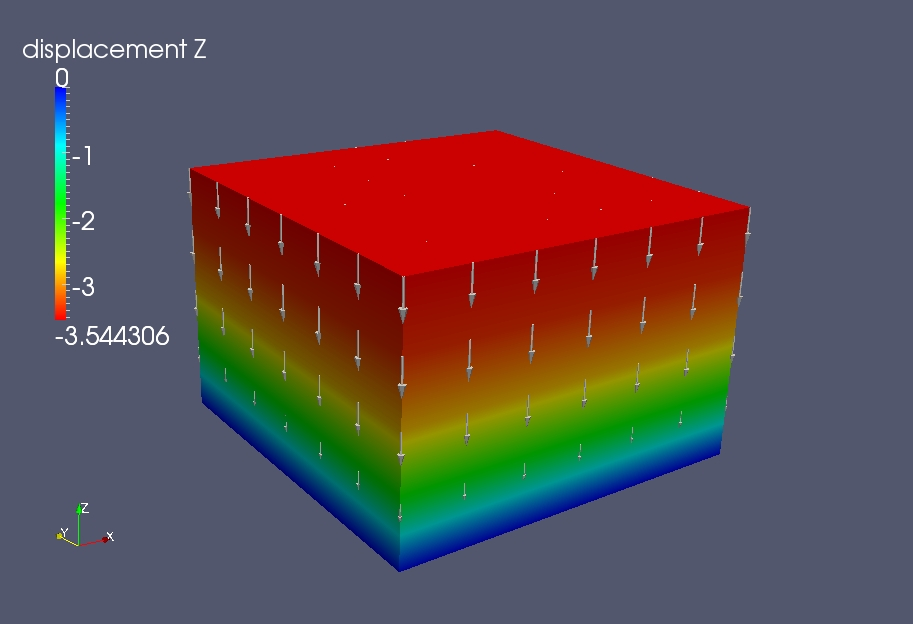
\includegraphics[width=10cm]{tutorials/3dhex8/figs/step15-displ-t200}
\par\end{centering}

\caption{Displacement field for example step15 at t = 200 years visualized
using ParaView. The z-component of the displacement field is shown
with the color contours, and the vectors show the computed displacements.\label{fig:step15-displ-t200}}


\end{figure}



\subsubsection{Step16 - Gravitational Body Forces with Initial Stresses}

The \texttt{step16.cfg} file defines a problem that is identical to
example step15, except that initial stresses are used to prevent the
initial large displacements due to 'turning on' gravity. Since all
normal stress components are given an initial stress of $\rho gh$,
the initial stress state is lithostatic, which is an appropriate condition
for many tectonic problems in the absence of tectonic stresses (e.g.,
McGarr \cite{McGarr:1988}). When compared to example step15, this
example should maintain a lithostatic state of stress for the entire
simulation, and displacements should remain essentially zero.

We set the gravity field, as in example step15, and we again use adaptive
time stepping with a generalized Maxwell rheology for the lower crust.
We provide values for the initial stress for both the upper and lower
crust. Since the materials have the same density, we are able to use
the same \texttt{SimpleDB} with a linear variation for both (see file
\texttt{examples/3d/hex8/spatialdb/initial\_stress.spatialdb}):
\begin{lyxcode}
\#~We~must~specify~initial~stresses~for~each~material.

\#~We~provide~a~filename~for~the~spatial~database~that~gives~the~stresses,

\#~and~we~change~the~query\_type~from~the~default~'nearest'~to~'linear'.

{[}pylithapp.timedependent.materials.upper\_crust{]}

db\_initial\_stress~=~spatialdata.spatialdb.SimpleDB

db\_initial\_stress.iohandler.filename~=~spatialdb/initial\_stress.spatialdb

db\_initial\_stress.query\_type~=~linear~\\
~\\


{[}pylithapp.timedependent.materials.lower\_crust{]}

db\_initial\_stress~=~spatialdata.spatialdb.SimpleDB

db\_initial\_stress.iohandler.filename~=~spatialdb/initial\_stress.spatialdb

db\_initial\_stress.query\_type~=~linear
\end{lyxcode}
Note that we use a \texttt{linear} \texttt{query\_type} rather than
the default type of \texttt{nearest}, so that a linear interpolation
is performed along the z-direction. When we have run the simulation,
the output VTK files will be contained in \texttt{examples/3d/hex8/output}
(all with a pvrefix of \texttt{step16}). Results using ParaView are
shown in Figure \vref{fig:step16-stress_xx-t200}.

\begin{figure}
\begin{centering}
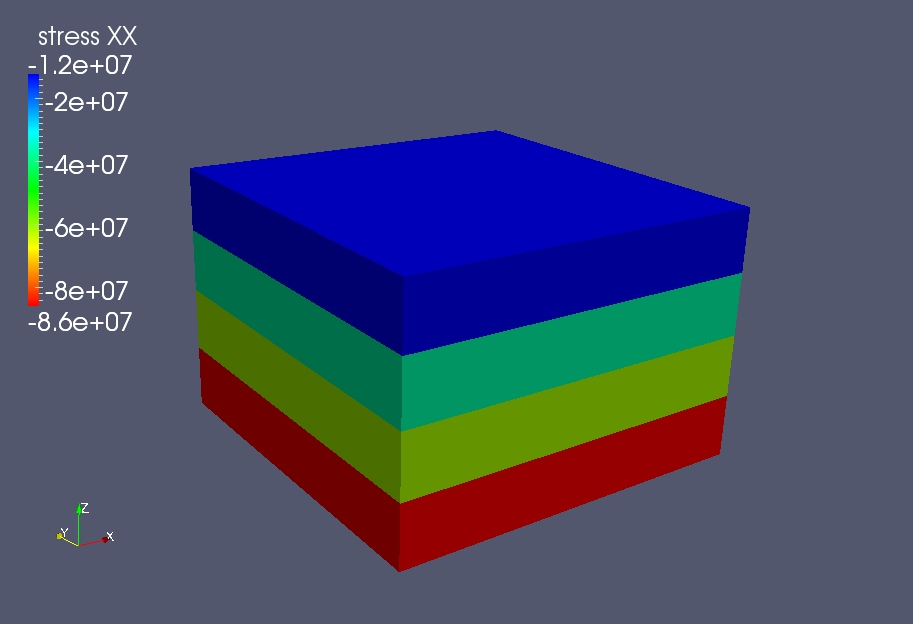
\includegraphics[width=10cm]{tutorials/3dhex8/figs/step16-stress_xx-t200}
\par\end{centering}

\caption{Stress field (xx-component) for example step16 at t = 200 years visualized
using ParaView. Note that for this example, Stress\_xx = Stress\_yy
= Stress\_zz, and there is no vertical displacement throughout the
simulation. Also note that the stresses appear as four layers since
we have used \texttt{CellFilterAvg} for material output.\label{fig:step16-stress_xx-t200}}
\end{figure}



\subsubsection{Step17 - Gravitational Body Forces with Small Strain}

The \texttt{step17.cfg} file defines a problem that is identical to
example step15, except that we now use a small strain formulation
(see Section \vref{sec:small:strain:formulation}). All of the problems
up to this point have assumed infinitesimal strain, meaning that the
change in shape of the domain during deformation is not taken into
account. In many problems it is important to consider the change in
shape of the domain. This is particularly important in many problems
involving gravitational body forces, since a change in shape of the
domain results in a different stress field. By examining the stress
and deformation fields for this example in comparison with those of
example step15, we can see what effect the infinitesimal strain approximation
has on our solution.

We set the gravity field, as in example step15 and again use adaptive
time stepping withs a generalized Maxwell rheology for the lower crust.
The only change is that we change the problem formulation from the
default \texttt{Implicit} to \texttt{ImplicitLgDeform}. Since the
large deformation formulation is nonlinear, PyLith automatically switches
the solver from the default \texttt{SolverLinear} to \texttt{SolverNonlinear}.
It is thus only necessary to change the formulation:
\begin{lyxcode}
{[}pylithapp.timedependent{]}

\#~Set~the~formulation~for~finite~strain.~The~default~solver~will

\#~automatically~be~switched~to~the~nonlinear~solver.

formulation~=~pylith.problems.ImplicitLgDeform
\end{lyxcode}
When we have run the simulation, the output VTK files will be contained
in \texttt{examples/3d/hex8/output} (all with a pvrefix of \texttt{step17}).
Results using ParaView are shown in Figure \vref{fig:step17-disp-t200}.

\begin{figure}
\begin{centering}
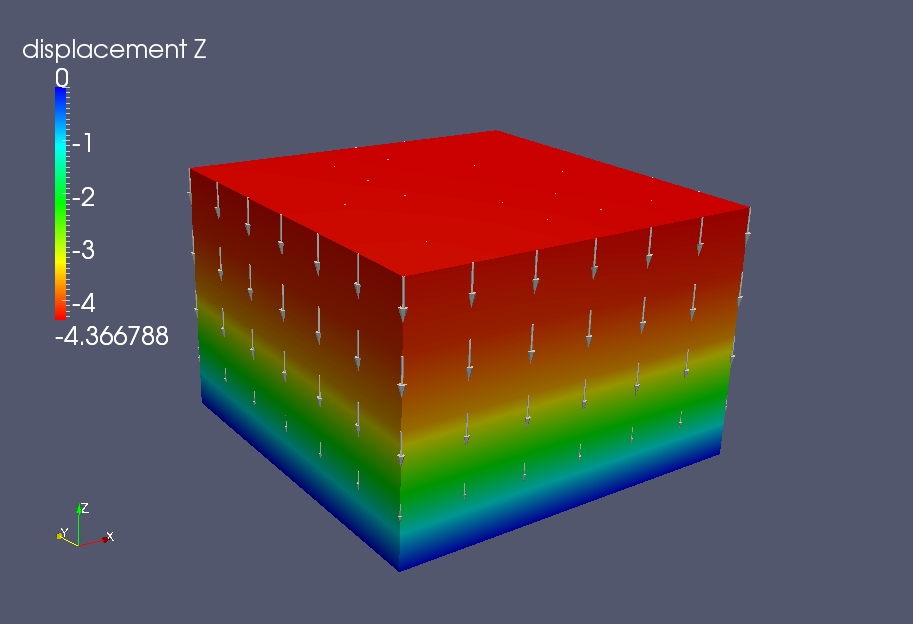
\includegraphics[width=10cm]{tutorials/3dhex8/figs/step17-displ-t200}
\par\end{centering}

\caption{Displacement field for example step17 at t = 200 years visualized
using ParaView. The z-component of the displacement field is shown
with the color contours, and the vectors show the computed displacements.
Note the larger displacements compared with example step15.\label{fig:step17-disp-t200}}
\end{figure}

